%Note di Ingegneria del Software
%Sommario: Definizione di SWE, Approccio

\cornell{Cos'è L'ingegneria del Software}{Nata nel 1968, ha l'obiettivo di Raccogliere, organizzare e consolidare la conoscenza necessaria a realizzare progetti software con massima efficienza ed efficacia. La materia non ha una base teorica certa, dato che è una disciplina molto giovane.}
\cornell{Secondo il Glossario IEEE}{L'approccio \begin{itemize}
	\item \textbf{Sistematico} \begin{itemize}
		\item Modo di lavorare metodico e rigoroso
		\item che studia, fa uso ed evolve le best practice di dominio
		\end{itemize}
	\item \textbf{Disciplinato} (Che segue regole fissate)
	\item \textbf{Quantificabile} (Che permette di misurare efficienza ed efficacia)
\end{itemize}\\
allo sviluppo, l'uso, la manutenzione ed il ritiro del software.}
\cornell{Metodo di studio}{Si va a costruire incrementalmente il proprio glossario \begin{enumerate}
	\item Basandolo inizialmente sulla teoria (individuando termini e significati)
	\item Consolidandolo con la prativa (applicazione e confronto critico con l'esperienza)
	\item Discutendo tale glossario con i colleghi (unione di conoscenze parziali, correzione reciproca).
\end{itemize}\\
Inoltre è necessario integrare le diapositive date nel corso con fonti e risorse autorevoli, in sessioni di studio personale.}
\cornell{Elementi di un progetto (gli "alphas" secondo SEMAT)}{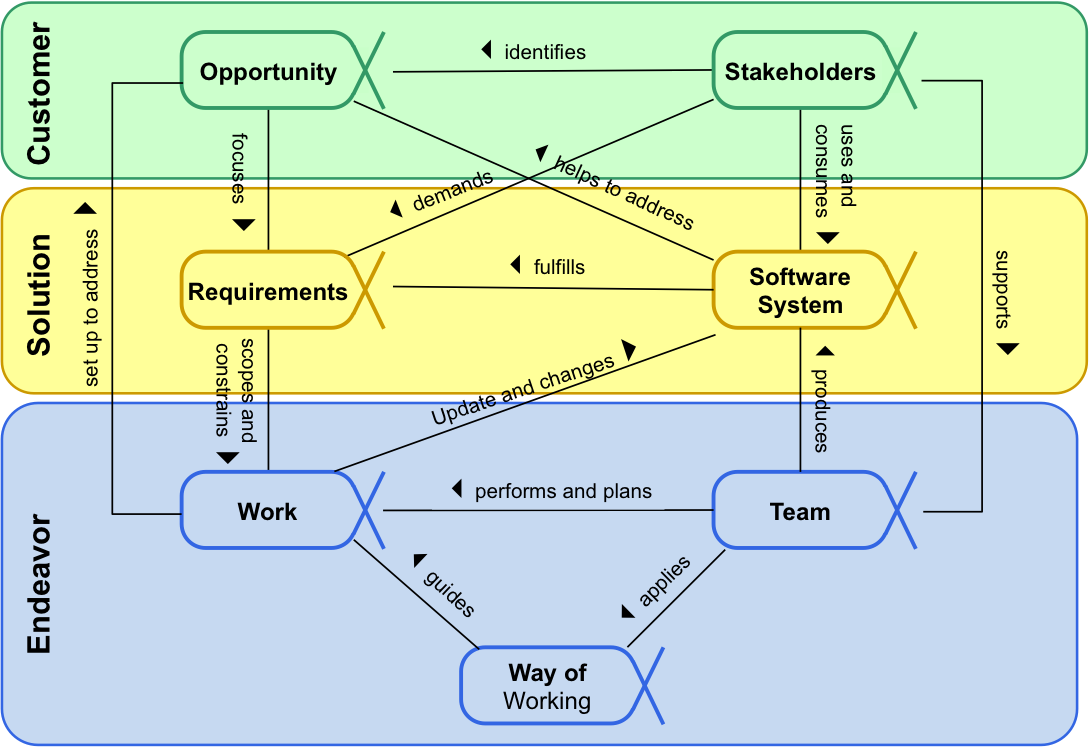
\includegraphics[scale=0.5]{images/1.png}}
\cornell{Opportunità}{Set di circostanze che rendono appropriata la produzione o il cambiamento di un sistema software.\\
In pratica è la ragione per la creazione di un nuovo (o diverso) sistema software. Rappresenta la comprensione condivisa delle necessità dello stakeholder (portatore di interesse) ed aiuta a formare i requisiti per il nuovo sistema software, dando giustificazione alla sua creazione.}
